\documentclass[11pt]{article}
\usepackage{geometry}                % See geometry.pdf to learn the layout options. There are lots.
\geometry{letterpaper}                   % ... or a4paper or a5paper or ... 
%\geometry{landscape}                % Activate for for rotated page geometry
%\usepackage[parfill]{parskip}    % Activate to begin paragraphs with an empty line rather than an indent
\usepackage{fancyhdr}
\usepackage{amsmath,amsfonts,amsthm,amssymb}
\usepackage{graphicx}
\usepackage{soul,color}
\usepackage{graphicx,float,wrapfig}
\usepackage{lastpage}
\usepackage{epstopdf}
\DeclareGraphicsRule{.tif}{png}{.png}{`convert #1 `dirname #1`/`basename #1 .tif`.png}

% Homework Specific Information
\newcommand{\hmwkTitle}{Homework 4}
\newcommand{\hmwkDueDate}{April 25, 2012}
\newcommand{\hmwkClass}{Computational Neuroscience}
\newcommand{\hmwkClassInstructor}{John Rinzel}
\newcommand{\hmwkAuthorName}{Raphael Sofaer}

% Setup the header and footer
\pagestyle{fancy}                                                       %
\lhead{\hmwkAuthorName}                                                 %
\rhead{\hmwkClass\ (\hmwkClassInstructor): \hmwkTitle}  %
\lfoot{\lastxmark}                                                      %
\cfoot{}                                                                %
\rfoot{Page\ \thepage\ of\ \pageref{LastPage}}                          %
\renewcommand\headrulewidth{0.4pt}                                      %
\renewcommand\footrulewidth{0.4pt}                                      %
\setlength{\headheight}{13.6pt}

\title{\large{\hmwkAuthorName}\vspace{0.1in}\\\textmd{\textbf{\hmwkClass:\ \hmwkTitle}}\\\normalsize\vspace{0.1in}\small{Due\ on\ \hmwkDueDate}\\\vspace{0.1in}\large{\textit{\hmwkClassInstructor}}\vspace{0.1in}}
\author{}
\date{}
  
\begin{document}
\maketitle

\section*{Short-Term Memory model with Adaptation: 1}
I based my Matlab script (run in Octave) on STM\_MF.m.  For the first run, I used $\gamma=2$ to match the graph in the homework description.\\
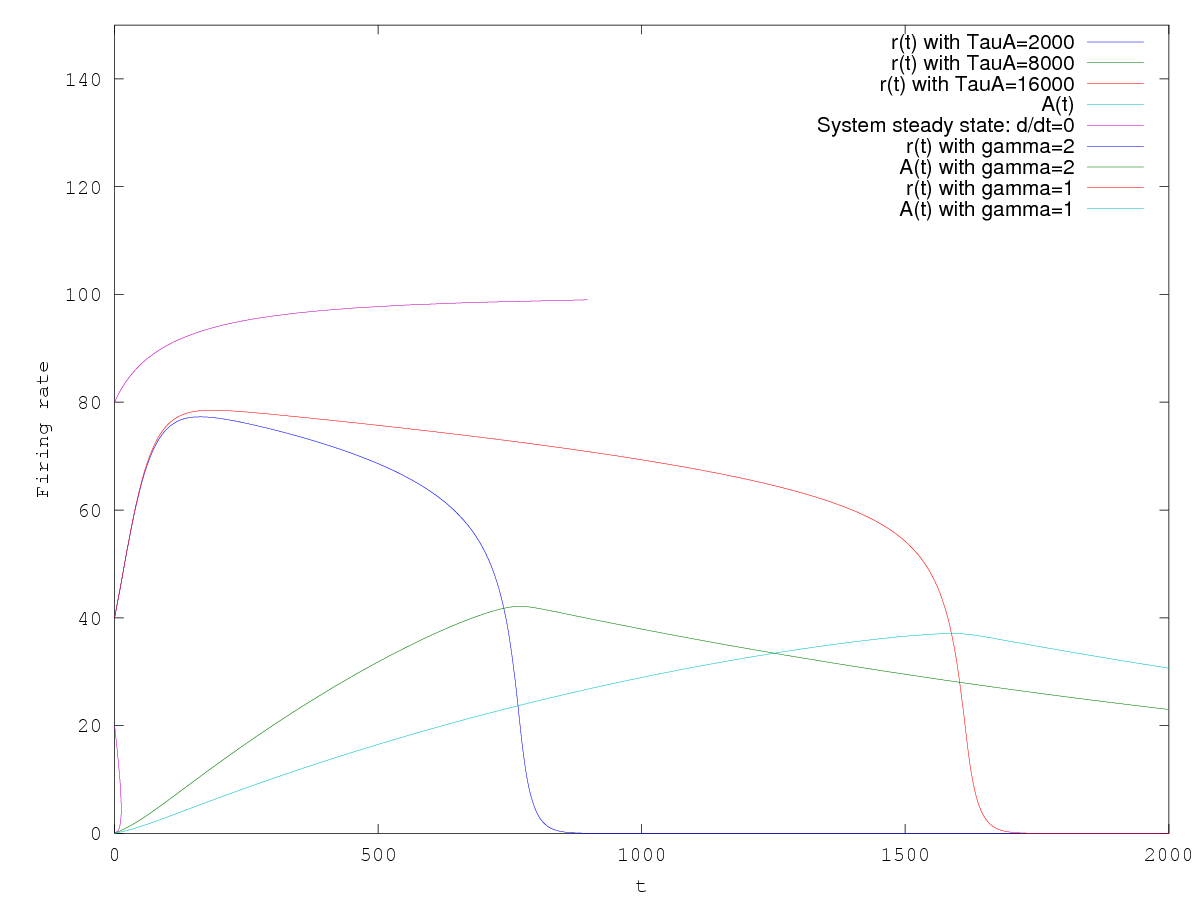
\includegraphics[width=6in]{1.png}\\
\section*{2}
For the second set of trials, I changed $\gamma$ to $1$.  As I increased $\tau_A$, the system slowed down.  A(t) changed more slowly, so it took longer for A(t) to increase to drive R(t) down, and it took longer for A(t) do decrease again after R(t) plummeted.  The shape of the curves was qualitatively similar, however.\\
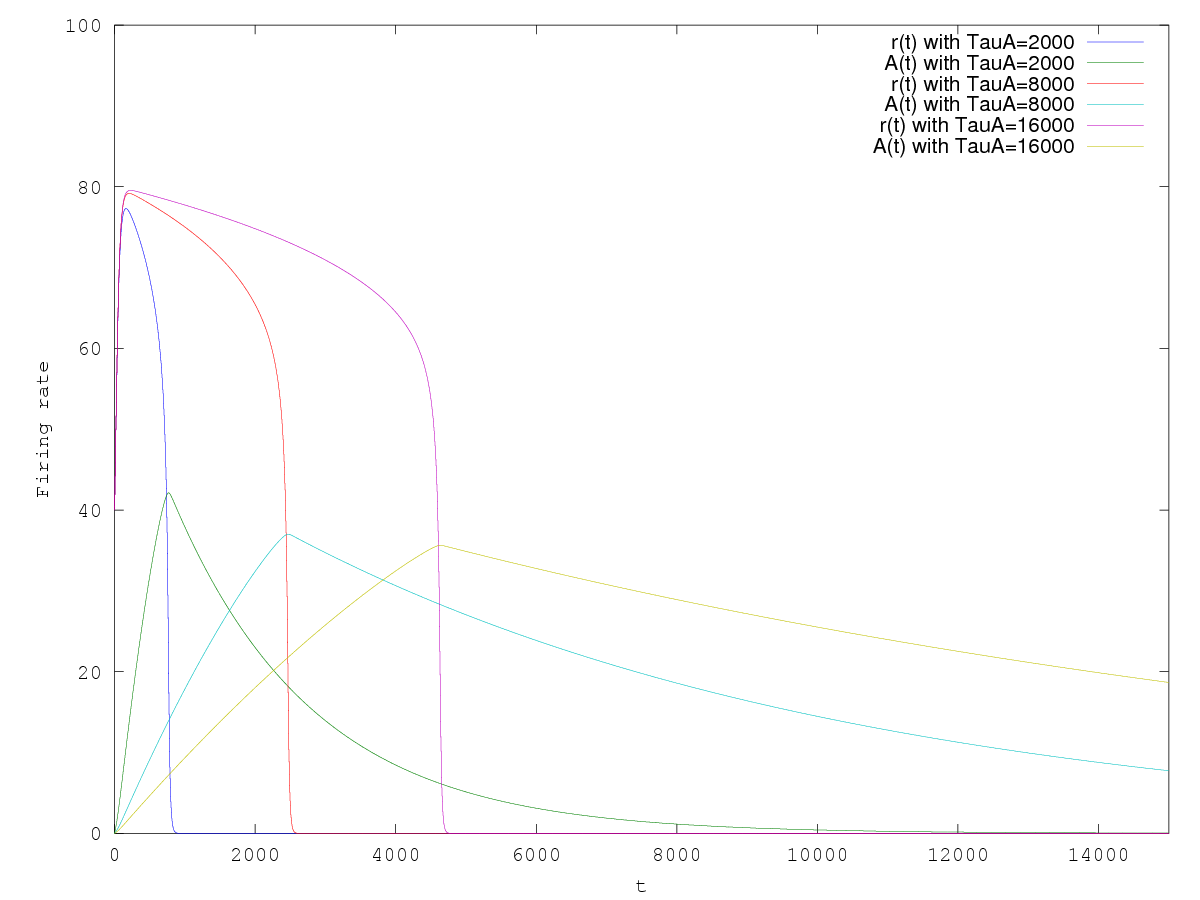
\includegraphics[width=6in]{2.png}\\

\newpage
\section*{3}
I approached finding the steady state curve analytically for individual values of r.  Given:
$\tau(dr/dt) = -r + S_{NR}(ar - A)$ (I = 0), we can set $dr/dt$ to 0 and calculate from there.
\begin{align*}
  r &= S_{NR}(ar-A)\\
  r &= \frac{M*(ar-A)^2}{\sigma^2 + (ar-A)^2}\\
  \delta &= (ar - A)^2\\
  r &= \frac{M*\delta}{\sigma^2 + \delta}\\
  r\sigma^2 + r\delta &= M*\delta\\
  \frac{r\sigma^2}{\delta} &= M-r\\
  \frac{1}{\delta} &= \frac{M-r}{r\sigma^2}\\
  \delta &= \frac{r\sigma^2}{M-r}\\
  A^2 - 2arA + a^2r^2 - \frac{r\sigma^2}{M-r} &= 0\\
  A &= \frac{\sigma}{\sqrt{M/r-1}} - a*r \\
\end{align*}
Since everything other than A is constant for a given r, this is a quadratic in A, easily solved.  In the graph below, we can see R jump to the upper part of the steady state, then fall to the bottom as the input disappears.\\
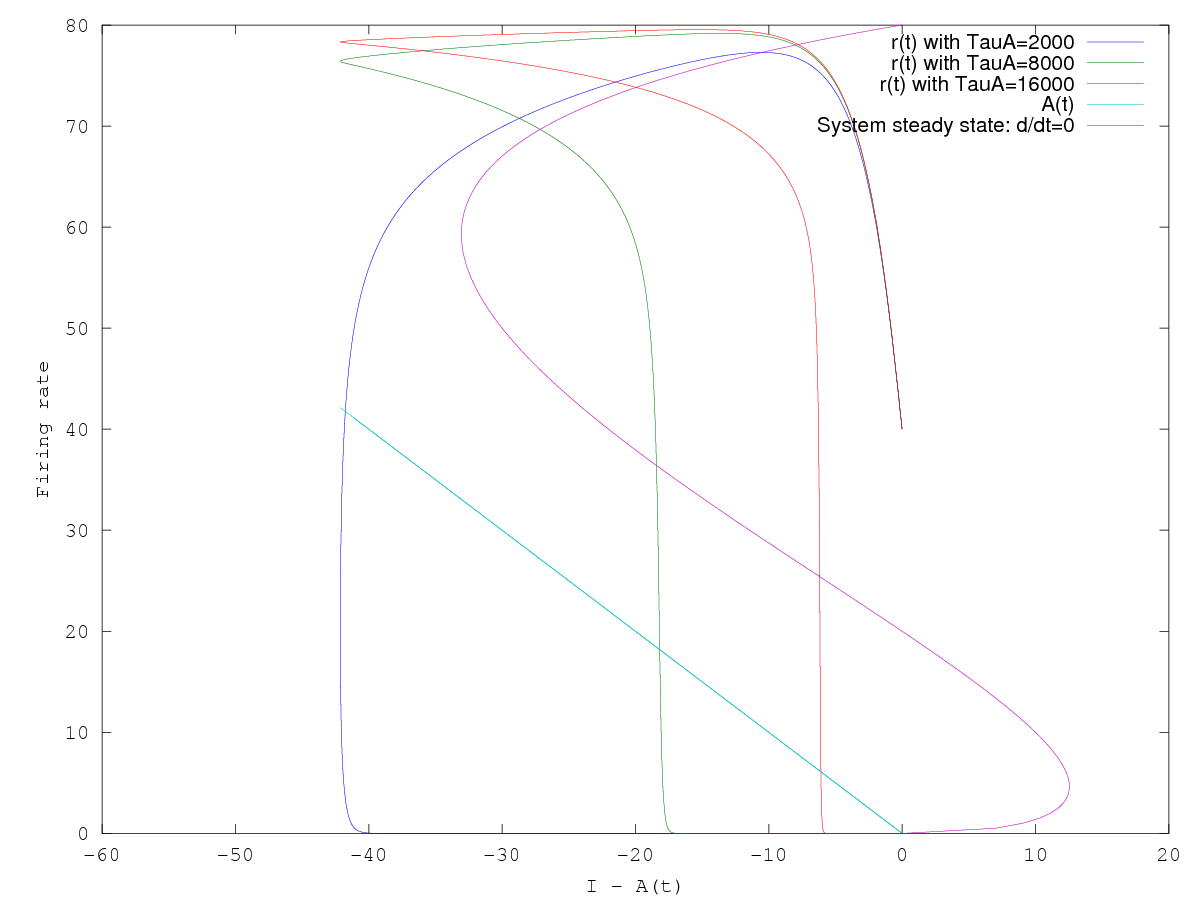
\includegraphics[width=6in]{3.png}\\

\newpage
\section*{4}
For varying the values of I, I set $\tau_A$ back to 2000.
In these time courses, instead of the firing rate falling
to nothing, the constant input current causes the neuron
to reach a steady state solid firing rate.
The steady state is about 62 for I=30, 72 for I=50,
and 78 for I=70.
For any given I, we could find what steady state it would 
go to by first checking the sign of $dr/dt$,
to know whether it would go to a zero or positive steady state,
then if $dr/dt>0$, we can solve for r in $r=S_{NA}(ar-A(r))$.\\
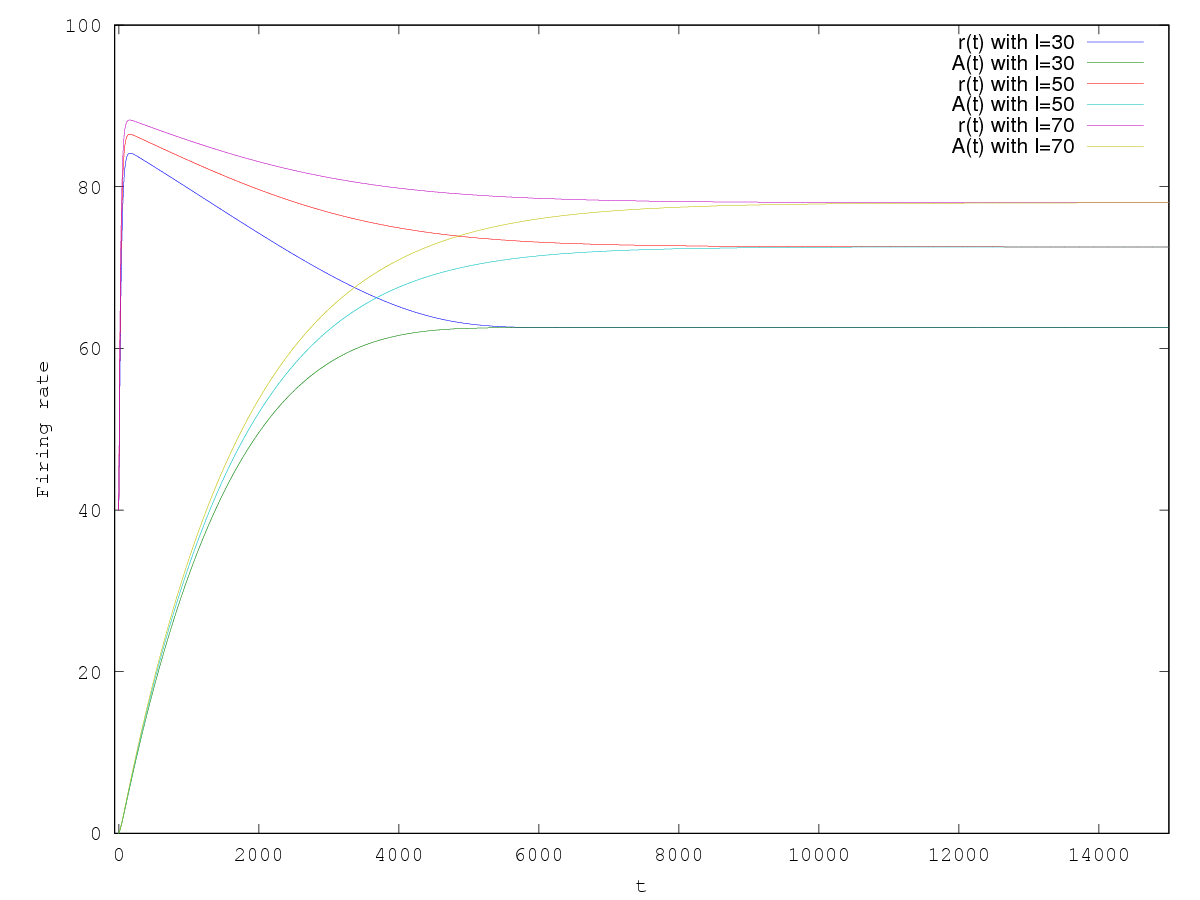
\includegraphics[width=6in]{4t.png}\\
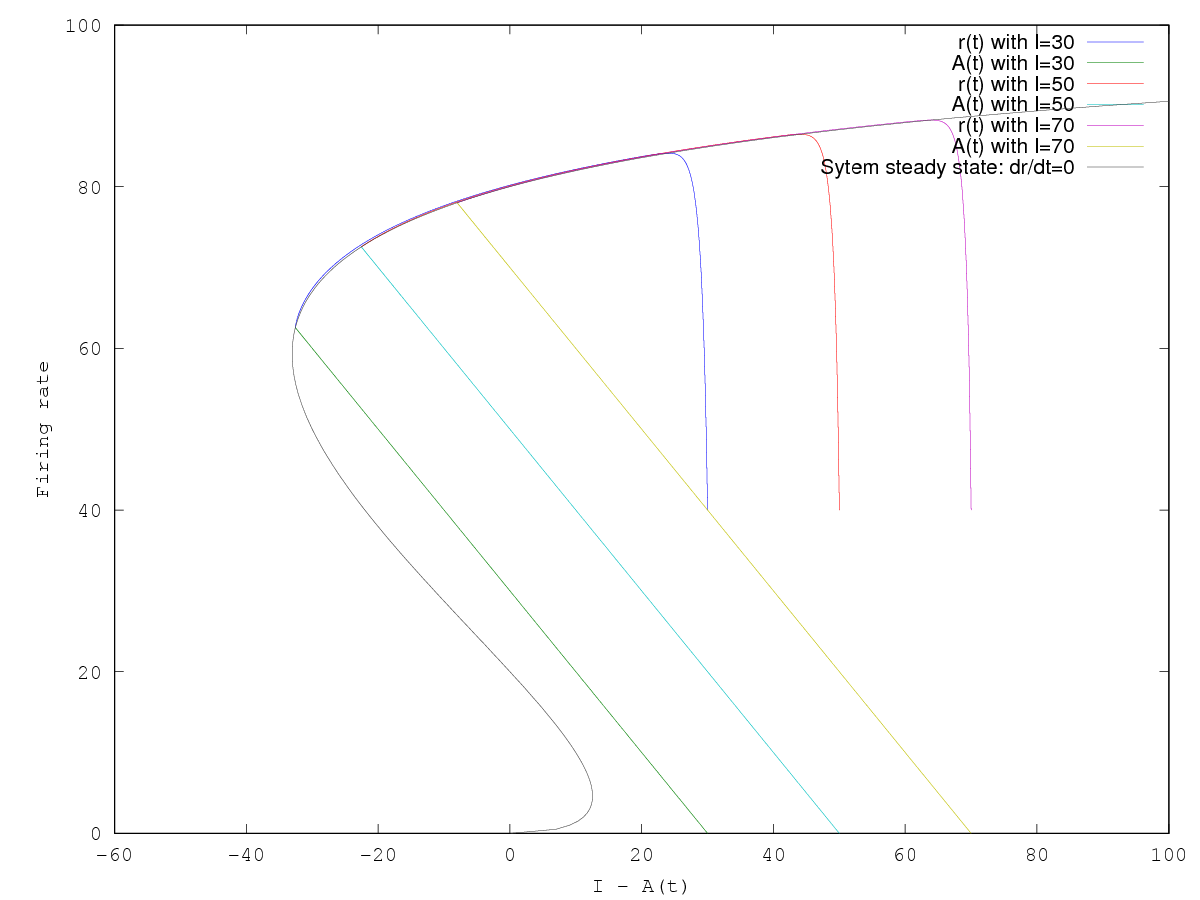
\includegraphics[width=6in]{4p.png}\\
\end{document}
